
% This LaTeX was auto-generated from MATLAB code.
% To make changes, update the MATLAB code and republish this document.

\documentclass{article}
\usepackage{graphicx}
\usepackage{color}

\sloppy
\definecolor{lightgray}{gray}{0.5}
\setlength{\parindent}{0pt}

\begin{document}

    
    
\subsection*{Contents}

\begin{itemize}
\setlength{\itemsep}{-1ex}
   \item AMSC 460 - HW11
   \item Problem 2 (
\end{itemize}


\subsection*{AMSC 460 - HW11}

\begin{verbatim}
clear all; format compact; close all; syms f(x) x y z
\end{verbatim}


\subsection*{Problem 2 (}

\begin{par}
Consider the function [f(x) = \ensuremath{\backslash}frac\{e\^{}\{3x\}\ensuremath{\backslash}sin(200x\^{}2)\}\{1+20x\^{}2\}\ensuremath{\backslash}]
\end{par} \vspace{1em}
\begin{verbatim}
syms x n
f(x) = (exp(3*x)*sin(200*x^2)/(1+20*x^2))
ezplot(f(x))
\end{verbatim}

        \color{lightgray} \begin{verbatim}f(x) =
(exp(3*x)*sin(200*x^2))/(20*x^2 + 1)
\end{verbatim} \color{black}
    
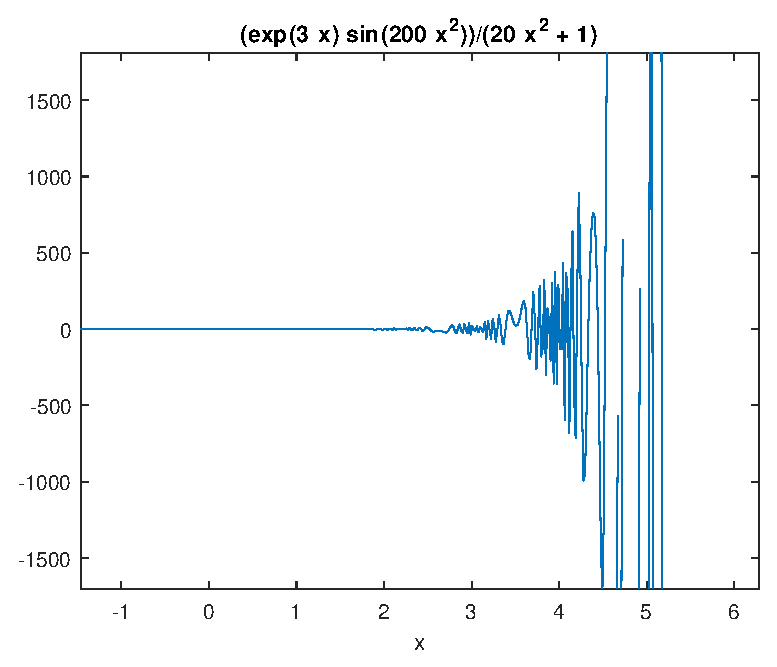
\includegraphics [width=4in]{HW14_01.eps}
\begin{verbatim}
z=6
test = 1: z
for k =1:z
    i = 0:test(k)
    xi = i/z
    spline(xi,fx)
end
\end{verbatim}

        \color{lightgray} \begin{verbatim}z =
     6
test =
     1     2     3     4     5     6
i =
     0     1
xi =
         0    0.1667
\end{verbatim} \color{black}
    
        \color{lightgray} \begin{verbatim}Unrecognized function or variable 'fx'.
Error in HW14 (line 18)
    spline(xi,fx)\end{verbatim} \color{black}
    \begin{par}
$|J(x)|\le 1$
\end{par} \vspace{1em}
\begin{par}
(b)Suppose we would like to approximate $J$ with a Chebyshev interpolant. Determine how many interpolation points  are required on the interval $[0,10]$ so that the error (in the max-norm) is no more than $10^{-6}$. [You don't have to write down the interpolant.]
\end{par} \vspace{1em}



\end{document}

